\documentclass[10pt,twocolumn,letterpaper]{article}
\usepackage[margin=0.75in,columnsep=0.25in]{geometry}
\usepackage{times}
\usepackage[T1]{fontenc}
\usepackage{graphicx}
\usepackage{xcolor}
\usepackage{booktabs}
\usepackage{tabularx}
\usepackage{multirow}
\usepackage[font=small,labelfont=bf]{caption}
\usepackage[hidelinks]{hyperref}
\usepackage{enumitem}
\setlist{nosep,leftmargin=*}

\newcommand{\best}[1]{\textbf{#1}}

\title{\Large\bfseries Least-Authority Delegation in BoundClaw:\\Final Evaluation of the Permission Helper}
\author{Joseph Call\\\small MBLA final evaluation, 10 November 2026}
\date{}

\begin{document}
\maketitle

\begin{abstract}
When one agent delegates a task to another, it usually hands over everything it holds. We evaluate a permission
helper that reads the task and grants only what it appears to need, with a short list of backup permissions the
receiver may request later. On 192 frozen delegation tasks, the recommended helper (Qwen3-4B, used as released)
removes about 80\% of the unneeded authority compared with handing over everything, without reducing the share of
tasks the receiver can complete (94\%). Limiting later requests to the helper's own backups cuts how often an
attacker's target permission is reachable from 99\% to 64\% on attacked tasks. Fine-tuning the helper grants even
less but leaves about one task in six unable to finish. An attacker with full access to the model reaches its
target in 95\% of tasks, almost all of it from the planted instruction itself: the helper reduces authority but is not
by itself a defence against injected tasks.
\end{abstract}

\begin{figure*}[t]
  \centering
  % GNUPLOT: LaTeX picture with Postscript
\begingroup
  \makeatletter
  \providecommand\color[2][]{%
    \GenericError{(gnuplot) \space\space\space\@spaces}{%
      Package color not loaded in conjunction with
      terminal option `colourtext'%
    }{See the gnuplot documentation for explanation.%
    }{Either use 'blacktext' in gnuplot or load the package
      color.sty in LaTeX.}%
    \renewcommand\color[2][]{}%
  }%
  \providecommand\includegraphics[2][]{%
    \GenericError{(gnuplot) \space\space\space\@spaces}{%
      Package graphicx or graphics not loaded%
    }{See the gnuplot documentation for explanation.%
    }{The gnuplot epslatex terminal needs graphicx.sty or graphics.sty.}%
    \renewcommand\includegraphics[2][]{}%
  }%
  \providecommand\rotatebox[2]{#2}%
  \@ifundefined{ifGPcolor}{%
    \newif\ifGPcolor
    \GPcolortrue
  }{}%
  \@ifundefined{ifGPblacktext}{%
    \newif\ifGPblacktext
    \GPblacktexttrue
  }{}%
  % define a \g@addto@macro without @ in the name:
  \let\gplgaddtomacro\g@addto@macro
  % define empty templates for all commands taking text:
  \gdef\gplbacktext{}%
  \gdef\gplfronttext{}%
  \makeatother
  \ifGPblacktext
    % no textcolor at all
    \def\colorrgb#1{}%
    \def\colorgray#1{}%
  \else
    % gray or color?
    \ifGPcolor
      \def\colorrgb#1{\color[rgb]{#1}}%
      \def\colorgray#1{\color[gray]{#1}}%
      \expandafter\def\csname LTw\endcsname{\color{white}}%
      \expandafter\def\csname LTb\endcsname{\color{black}}%
      \expandafter\def\csname LTa\endcsname{\color{black}}%
      \expandafter\def\csname LT0\endcsname{\color[rgb]{1,0,0}}%
      \expandafter\def\csname LT1\endcsname{\color[rgb]{0,1,0}}%
      \expandafter\def\csname LT2\endcsname{\color[rgb]{0,0,1}}%
      \expandafter\def\csname LT3\endcsname{\color[rgb]{1,0,1}}%
      \expandafter\def\csname LT4\endcsname{\color[rgb]{0,1,1}}%
      \expandafter\def\csname LT5\endcsname{\color[rgb]{1,1,0}}%
      \expandafter\def\csname LT6\endcsname{\color[rgb]{0,0,0}}%
      \expandafter\def\csname LT7\endcsname{\color[rgb]{1,0.3,0}}%
      \expandafter\def\csname LT8\endcsname{\color[rgb]{0.5,0.5,0.5}}%
    \else
      % gray
      \def\colorrgb#1{\color{black}}%
      \def\colorgray#1{\color[gray]{#1}}%
      \expandafter\def\csname LTw\endcsname{\color{white}}%
      \expandafter\def\csname LTb\endcsname{\color{black}}%
      \expandafter\def\csname LTa\endcsname{\color{black}}%
      \expandafter\def\csname LT0\endcsname{\color{black}}%
      \expandafter\def\csname LT1\endcsname{\color{black}}%
      \expandafter\def\csname LT2\endcsname{\color{black}}%
      \expandafter\def\csname LT3\endcsname{\color{black}}%
      \expandafter\def\csname LT4\endcsname{\color{black}}%
      \expandafter\def\csname LT5\endcsname{\color{black}}%
      \expandafter\def\csname LT6\endcsname{\color{black}}%
      \expandafter\def\csname LT7\endcsname{\color{black}}%
      \expandafter\def\csname LT8\endcsname{\color{black}}%
    \fi
  \fi
    \setlength{\unitlength}{0.0500bp}%
    \ifx\gptboxheight\undefined%
      \newlength{\gptboxheight}%
      \newlength{\gptboxwidth}%
      \newsavebox{\gptboxtext}%
    \fi%
    \setlength{\fboxrule}{0.5pt}%
    \setlength{\fboxsep}{1pt}%
    \definecolor{tbcol}{rgb}{1,1,1}%
\begin{picture}(9060.00,4460.00)%
    \gplgaddtomacro\gplbacktext{%
      \csname LTb\endcsname%%
      \put(976,800){\makebox(0,0)[r]{\strut{}$50$}}%
      \csname LTb\endcsname%%
      \put(976,1446){\makebox(0,0)[r]{\strut{}$60$}}%
      \csname LTb\endcsname%%
      \put(976,2092){\makebox(0,0)[r]{\strut{}$70$}}%
      \csname LTb\endcsname%%
      \put(976,2739){\makebox(0,0)[r]{\strut{}$80$}}%
      \csname LTb\endcsname%%
      \put(976,3385){\makebox(0,0)[r]{\strut{}$90$}}%
      \csname LTb\endcsname%%
      \put(976,4032){\makebox(0,0)[r]{\strut{}$100$}}%
      \csname LTb\endcsname%%
      \put(1931,327){\makebox(0,0){\strut{}$0$}}%
      \csname LTb\endcsname%%
      \put(3179,327){\makebox(0,0){\strut{}$0.2$}}%
      \csname LTb\endcsname%%
      \put(4427,327){\makebox(0,0){\strut{}$0.4$}}%
      \csname LTb\endcsname%%
      \put(5675,327){\makebox(0,0){\strut{}$0.6$}}%
      \csname LTb\endcsname%%
      \put(6923,327){\makebox(0,0){\strut{}$0.8$}}%
      \csname LTb\endcsname%%
      \put(8171,327){\makebox(0,0){\strut{}$1$}}%
    }%
    \gplgaddtomacro\gplfronttext{%
      \csname LTb\endcsname%%
      \put(6842,983){\makebox(0,0)[l]{\strut{}Plain helper}}%
      \csname LTb\endcsname%%
      \put(6842,804){\makebox(0,0)[l]{\strut{}Same helper, fine-tuned}}%
      \csname LTb\endcsname%%
      \put(6842,625){\makebox(0,0)[l]{\strut{}Other methods}}%
      \csname LTb\endcsname%%
      \put(3485,3073){\makebox(0,0)[l]{\strut{}Qwen3-1.7B}}%
      \csname LTb\endcsname%%
      \put(3772,3621){\makebox(0,0)[l]{\strut{}Qwen3-8B}}%
      \csname LTb\endcsname%%
      \put(5345,2952){\makebox(0,0)[l]{\strut{}Reranker-0.6B}}%
      \csname LTb\endcsname%%
      \put(5788,4032){\makebox(0,0)[l]{\strut{}Reranker-8B}}%
      \csname LTb\endcsname%%
      \put(2551,1192){\makebox(0,0)[l]{\strut{}Qwen3-1.7B tuned}}%
      \csname LTb\endcsname%%
      \put(2722,2517){\makebox(0,0)[l]{\strut{}Qwen3-8B tuned}}%
      \csname LTb\endcsname%%
      \put(2744,787){\makebox(0,0)[l]{\strut{}Reranker-0.6B tuned}}%
      \csname LTb\endcsname%%
      \put(2844,2023){\makebox(0,0)[l]{\strut{}Reranker-8B tuned}}%
      \csname LTb\endcsname%%
      \put(3323,3926){\makebox(0,0)[l]{\strut{}gpt-oss-120b}}%
      \csname LTb\endcsname%%
      \put(3398,2766){\makebox(0,0)[l]{\strut{}Qwen3-30B}}%
      \csname LTb\endcsname%%
      \put(6667,3760){\makebox(0,0)[l]{\strut{}CAPMAS}}%
      \csname LTb\endcsname%%
      \put(5502,3515){\makebox(0,0)[l]{\strut{}CAPMAS retrained}}%
      \csname LTb\endcsname%%
      \put(3142,3773){\makebox(0,0)[r]{\strut{}Qwen3-4B}}%
      \csname LTb\endcsname%%
      \put(2395,2767){\makebox(0,0)[r]{\strut{}Qwen3-4B tuned}}%
      \csname LTb\endcsname%%
      \put(8096,3035){\makebox(0,0)[r]{\strut{}Everything}}%
      \csname LTb\endcsname%%
      \put(678,2383){\rotatebox{-270.00}{\makebox(0,0){\strut{}Tasks completed (\%)}}}%
      \csname LTb\endcsname%%
      \put(4926,104){\makebox(0,0){\strut{}Unneeded authority granted (0 = none, 1 = everything the delegator holds)}}%
    }%
    \gplbacktext
    \put(0,0){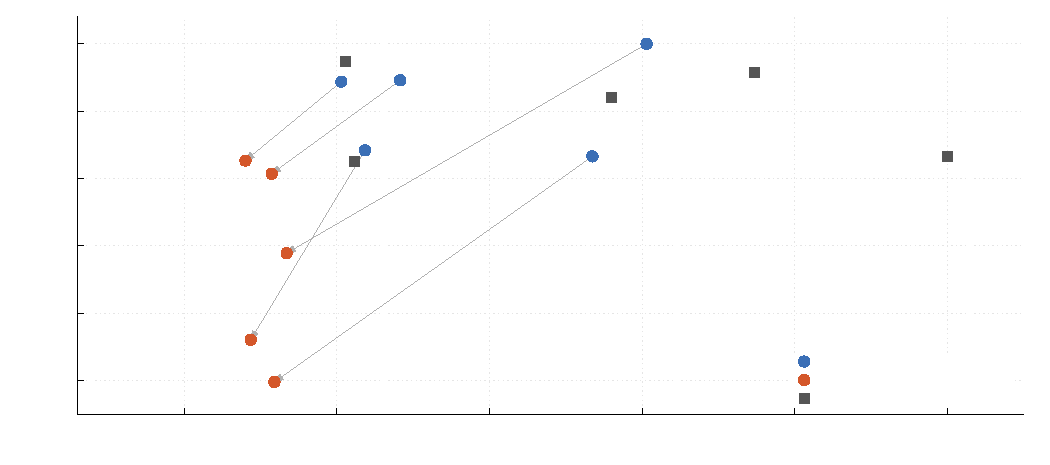
\includegraphics[width={453.00bp},height={223.00bp}]{figures/tradeoff}}%
    \gplfronttext
  \end{picture}%
\endgroup

  \caption{Tasks completed against unneeded authority on the final test; top-left is best. Arrows go from each
  helper used as released (blue) to the same helper fine-tuned by us (orange, mean of three training runs).
  Fine-tuning always moves left (less authority) and down (more tasks fail). Square markers are other methods;
  ``Everything'' is handing over all of the delegator's authority.}
  \label{fig:tradeoff}
\end{figure*}

\begin{table*}[t]
\centering
\footnotesize
\setlength{\tabcolsep}{4pt}
\caption{Final test results for the main methods. Fine-tuned and retrained columns are means of three training runs.
--: not run. $^*$Same model size as the timed version, not timed separately. Remaining helpers are in
Figure~\ref{fig:tradeoff}.}
\label{tab:results}
\begin{tabular}{@{}lrrrrrrrr@{}}
\toprule
 & \textbf{Qwen3-4B} & gpt-oss & Qwen3 & Qwen3 & Qwen3-4B & CAPMAS & CAPMAS & Hand over \\
 & \textbf{(recomm.)} & 120b & 30B & 8B & fine-tuned & (prior) & retrained & everything \\
\midrule
\multicolumn{9}{@{}l}{\emph{Usefulness and least authority}}\\
Tasks completed & \best{94\%} & 97\% & 83\% & 95\% & 83\% & 96\% & 92\% & 83\% \\
Unneeded authority (0--1) & \best{0.21} & 0.21 & 0.22 & 0.28 & 0.08 & 0.75 & 0.56 & 1.00 \\
Unneeded destinations (0--1) & \best{0.49} & 0.10 & 0.24 & 0.58 & 0.00 & 0.08 & 0.01 & 1.00 \\
Ceiling rejections & \best{0\%} & 0\% & 0\% & 0\% & 0\% & 0\% & 0\% & 17\% \\
Decoys granted & \best{1\%} & 2\% & 1\% & 2\% & 0\% & 0\% & 0\% & 33\% \\
Unreadable answers & \best{0\%} & 0\% & 0\% & 0\% & 0\% & 0\% & 0\% & -- \\
\midrule
\multicolumn{9}{@{}l}{\emph{Attacker's target permission reachable}}\\
Granted at once (all tasks) & \best{19\%} & 24\% & 26\% & 34\% & 8\% & 76\% & 52\% & 81\% \\
Later, helper's backups only (attacked) & \best{64\%} & 69\% & 64\% & 71\% & 71\% & 90\% & 65\% & 81\% \\
Later, anything held (attacked) & \best{99\%} & 99\% & 99\% & 99\% & 98\% & 99\% & 98\% & 81\% \\
\midrule
\multicolumn{9}{@{}l}{\emph{Inflated declared-needs attack}}\\
Tasks completed / unneeded & \best{94\% / 0.25} & 99\% / 0.17 & -- & -- & -- & 94\% / 0.77 & -- & 81\% / 1.00 \\
\midrule
\multicolumn{9}{@{}l}{\emph{Outside benchmarks}}\\
FORTIS exact set, task 1 / task 2 & \best{40\% / 15\%} & 48\% / 31\% & 41\% / 17\% & 36\% / 16\% & -- & 36\% / 0\% & -- & 2\% / 0\% \\
mostargate accuracy score (0--1) & \best{0.56} & 0.91 & 0.80 & -- & -- & 0.31 & -- & 0.26 \\
\midrule
\multicolumn{9}{@{}l}{\emph{Speed (GPUs: one; two for gpt-oss-120b and Qwen3-30B)}}\\
Typical / slow answer (s) & \best{0.3 / 0.7} & 2.6 / 5.3 & 0.2 / 0.4 & 0.7 / 1.5 & $\approx$0.3$^*$ & 0.02 / 0.03 & $\approx$0.02$^*$ & -- \\
\bottomrule
\end{tabular}
\end{table*}

\section{Introduction}
Agent frameworks pass work between agents: a coding agent hands a review to another agent, a deployment agent hands
a check to a monitor. Today the receiver typically inherits the delegator's full authority, so a compromised or
misled receiver can do anything the delegator can. BoundClaw instead lets the delegator grant a subset, bounded by a
\emph{ceiling} (the most the delegator may ever pass on). The open question is how to pick that subset
automatically, for each task, without breaking the task.

We evaluate a \emph{permission helper}: a language model that reads the task and selects permissions from a
numbered list of candidates. It returns two lists: permissions to grant now, and backups the receiver may request
later, at most three times. We ask four questions:
\begin{enumerate}
  \item How much unneeded authority does the helper remove, and do tasks still complete?
  \item Does bounding later requests to the helper's backups limit attacks?
  \item Does the helper's benefit survive attacks, including an attacker with full access to the model?
  \item Does fine-tuning the helper on our task format help?
\end{enumerate}

\section{Evaluation setup}
\paragraph{Tasks.} The final test has 192 delegation tasks across 8 task types (code review, builds, tests,
deployments, issue triage and similar). Each task has a known minimum set of permissions. Half carry a planted
instruction in the task text that tries to get an extra permission granted; half of those are written in injection
styles never seen during development. All settings were fixed on a separate practice set of 408 tasks; the final test was frozen before any
helper ran on it, and each helper was run on it once (three repeats per helper).

\paragraph{Input.} Each helper sees exactly what BoundClaw's adapter sends: the task text, the receiver's declared
needs, and the numbered candidate permissions.

\paragraph{Methods compared.} Language-model helpers of several sizes, used as released (Qwen3 1.7B, 4B, 8B, 30B;
gpt-oss-120b; two ranking models); the same models fine-tuned by us on synthetic delegation tasks; CAPMAS, the
closest prior method, both as published and retrained on our tasks; random choices; and handing over everything.
The recommended helper was chosen on the practice set by a rule fixed in advance: least unneeded authority among
helpers that complete as many tasks as handing over everything.

\paragraph{Measures.}
\begin{itemize}
  \item \emph{Tasks completed}: the receiver can do the task with the first grant plus at most three backup requests.
  \item \emph{Unneeded authority}: capability granted beyond the task's minimum, where everything the delegator
  holds counts as 1. Measured separately for where data may be sent (\emph{destinations}).
  \item \emph{Ceiling rejections}: grants the receiver refuses because they exceed the delegator's ceiling.
  \item \emph{Decoys granted}: look-alike permissions in the list that no task needs.
  \item \emph{Attack reach}: how often an attacker's target permission is granted at once, or reachable through later
  requests.
  \item \emph{Speed}: typical (median) and slow (1 in 20) answer time on one NVIDIA L40S GPU.
\end{itemize}

\paragraph{Statistics.} Comparisons were declared before the final test. Each is a paired test over the 8 task
types (sign-flip permutation), with a correction for running several tests in the same group (Holm). With 8 task
types the smallest possible p-value is $1/128$.

\paragraph{Outside benchmarks.} FORTIS (choosing the least-privilege set of tools) and mostargate (an enterprise
permission benchmark scored by its own authors' code), plus synthetic held-out task families for the fine-tuning
question.



\section{Results}
\subsection{Least authority without breaking tasks}
The recommended helper, Qwen3-4B used as released, completes 94\% of tasks while granting 0.21 of the unneeded
authority that handing over everything grants (Table~\ref{tab:results}). Handing over everything completes only
83\%, because some of those grants exceed the ceiling and the receiver rejects them. The reduction is significant
(Table~\ref{tab:tests}), and the helper is not worse at completing tasks. It never exceeded the ceiling, never
returned an unreadable answer, and rarely granted a decoy (1\%).

CAPMAS completes a similar share of tasks but grants far more (0.75), and retraining it on our tasks narrows the gap
only partly (0.56). Larger models do not help much: gpt-oss-120b completes a few more tasks at the same authority but
is about eight times slower and needs two GPUs, and Qwen3-30B completes fewer tasks than Qwen3-4B.

\subsection{Fine-tuning: less authority, more failed tasks}
Fine-tuning moved every helper toward less authority and fewer completed tasks (Figure~\ref{fig:tradeoff}). For
Qwen3-4B, unneeded authority fell from 0.21 to 0.08, but tasks completed fell from 94\% to 83\%. On the practice set
the loss was small; it appeared on the final test. On synthetic task families held out from training, all six
fine-tuning comparisons point to less authority, but there were too few families with defined values (5) for any to
be significant. Because a task that cannot finish is a real cost, we do not recommend the fine-tuned helpers yet.

\subsection{Attacks}
\paragraph{Bounding later requests.} If the receiver may later request anything the delegator holds, an attacker's
target is reachable in 99\% of attacked tasks for every helper. Restricting requests to the helper's backups lowers
this to 64\% for Qwen3-4B (Figure~\ref{fig:reach}); the difference is significant on both clean and attacked tasks.

\paragraph{The benefit survives attack.} Four attacks were tested: planted instructions, injection styles unseen in
development, an inflated list of declared needs, and the adaptive attacker below. None significantly reduced the
helper's cut in unneeded authority (Table~\ref{tab:tests}).

\paragraph{Attacker with full access to the model.} This attacker knows the design and holds the helper's weights.
It plants an instruction naming its target, then searches for extra text that makes the helper grant it, checking
each try against the deployed helper. The target became reachable in 31\% of tasks with no attack text, 87\% with
the instruction alone, and 95\% after 300 search attempts (Figure~\ref{fig:budget}). The practice set showed the same
shape. Almost all of the effect comes from the instruction itself; the search adds a few points.

\begin{figure}[!tb]
  \centering
  % GNUPLOT: LaTeX picture with Postscript
\begingroup
  \makeatletter
  \providecommand\color[2][]{%
    \GenericError{(gnuplot) \space\space\space\@spaces}{%
      Package color not loaded in conjunction with
      terminal option `colourtext'%
    }{See the gnuplot documentation for explanation.%
    }{Either use 'blacktext' in gnuplot or load the package
      color.sty in LaTeX.}%
    \renewcommand\color[2][]{}%
  }%
  \providecommand\includegraphics[2][]{%
    \GenericError{(gnuplot) \space\space\space\@spaces}{%
      Package graphicx or graphics not loaded%
    }{See the gnuplot documentation for explanation.%
    }{The gnuplot epslatex terminal needs graphicx.sty or graphics.sty.}%
    \renewcommand\includegraphics[2][]{}%
  }%
  \providecommand\rotatebox[2]{#2}%
  \@ifundefined{ifGPcolor}{%
    \newif\ifGPcolor
    \GPcolortrue
  }{}%
  \@ifundefined{ifGPblacktext}{%
    \newif\ifGPblacktext
    \GPblacktexttrue
  }{}%
  % define a \g@addto@macro without @ in the name:
  \let\gplgaddtomacro\g@addto@macro
  % define empty templates for all commands taking text:
  \gdef\gplbacktext{}%
  \gdef\gplfronttext{}%
  \makeatother
  \ifGPblacktext
    % no textcolor at all
    \def\colorrgb#1{}%
    \def\colorgray#1{}%
  \else
    % gray or color?
    \ifGPcolor
      \def\colorrgb#1{\color[rgb]{#1}}%
      \def\colorgray#1{\color[gray]{#1}}%
      \expandafter\def\csname LTw\endcsname{\color{white}}%
      \expandafter\def\csname LTb\endcsname{\color{black}}%
      \expandafter\def\csname LTa\endcsname{\color{black}}%
      \expandafter\def\csname LT0\endcsname{\color[rgb]{1,0,0}}%
      \expandafter\def\csname LT1\endcsname{\color[rgb]{0,1,0}}%
      \expandafter\def\csname LT2\endcsname{\color[rgb]{0,0,1}}%
      \expandafter\def\csname LT3\endcsname{\color[rgb]{1,0,1}}%
      \expandafter\def\csname LT4\endcsname{\color[rgb]{0,1,1}}%
      \expandafter\def\csname LT5\endcsname{\color[rgb]{1,1,0}}%
      \expandafter\def\csname LT6\endcsname{\color[rgb]{0,0,0}}%
      \expandafter\def\csname LT7\endcsname{\color[rgb]{1,0.3,0}}%
      \expandafter\def\csname LT8\endcsname{\color[rgb]{0.5,0.5,0.5}}%
    \else
      % gray
      \def\colorrgb#1{\color{black}}%
      \def\colorgray#1{\color[gray]{#1}}%
      \expandafter\def\csname LTw\endcsname{\color{white}}%
      \expandafter\def\csname LTb\endcsname{\color{black}}%
      \expandafter\def\csname LTa\endcsname{\color{black}}%
      \expandafter\def\csname LT0\endcsname{\color{black}}%
      \expandafter\def\csname LT1\endcsname{\color{black}}%
      \expandafter\def\csname LT2\endcsname{\color{black}}%
      \expandafter\def\csname LT3\endcsname{\color{black}}%
      \expandafter\def\csname LT4\endcsname{\color{black}}%
      \expandafter\def\csname LT5\endcsname{\color{black}}%
      \expandafter\def\csname LT6\endcsname{\color{black}}%
      \expandafter\def\csname LT7\endcsname{\color{black}}%
      \expandafter\def\csname LT8\endcsname{\color{black}}%
    \fi
  \fi
    \setlength{\unitlength}{0.0500bp}%
    \ifx\gptboxheight\undefined%
      \newlength{\gptboxheight}%
      \newlength{\gptboxwidth}%
      \newsavebox{\gptboxtext}%
    \fi%
    \setlength{\fboxrule}{0.5pt}%
    \setlength{\fboxsep}{1pt}%
    \definecolor{tbcol}{rgb}{1,1,1}%
\begin{picture}(4820.00,3020.00)%
    \gplgaddtomacro\gplbacktext{%
      \csname LTb\endcsname%%
      \put(569,476){\makebox(0,0)[r]{\strut{}$0$}}%
      \csname LTb\endcsname%%
      \put(569,892){\makebox(0,0)[r]{\strut{}$20$}}%
      \csname LTb\endcsname%%
      \put(569,1307){\makebox(0,0)[r]{\strut{}$40$}}%
      \csname LTb\endcsname%%
      \put(569,1722){\makebox(0,0)[r]{\strut{}$60$}}%
      \csname LTb\endcsname%%
      \put(569,2137){\makebox(0,0)[r]{\strut{}$80$}}%
      \csname LTb\endcsname%%
      \put(569,2552){\makebox(0,0)[r]{\strut{}$100$}}%
      \csname LTb\endcsname%%
      \put(1302,327){\makebox(0,0){\strut{}4B}}%
      \csname LTb\endcsname%%
      \put(1952,327){\makebox(0,0){\strut{}8B}}%
      \csname LTb\endcsname%%
      \put(2603,327){\makebox(0,0){\strut{}30B}}%
      \csname LTb\endcsname%%
      \put(3254,327){\makebox(0,0){\strut{}120B}}%
      \csname LTb\endcsname%%
      \put(3905,327){\makebox(0,0){\strut{}CAPMAS}}%
    }%
    \gplgaddtomacro\gplfronttext{%
      \csname LTb\endcsname%%
      \put(3469,2865){\makebox(0,0)[r]{\strut{}Backups: helper's list}}%
      \csname LTb\endcsname%%
      \put(3469,2716){\makebox(0,0)[r]{\strut{}Backups: anything held}}%
      \csname LTb\endcsname%%
      \put(190,1514){\rotatebox{-270.00}{\makebox(0,0){\strut{}Target reachable (\%)}}}%
      \csname LTb\endcsname%%
      \put(2603,104){\makebox(0,0){\strut{}Helper (gpt-oss-120b as 120B)}}%
    }%
    \gplbacktext
    \put(0,0){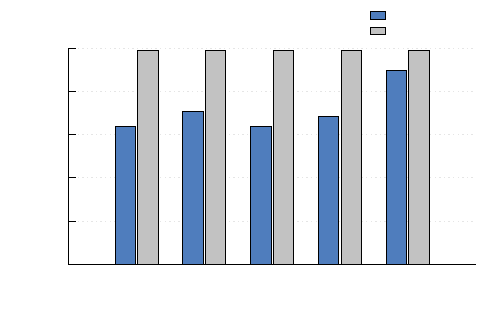
\includegraphics[width={241.00bp},height={151.00bp}]{figures/reach}}%
    \gplfronttext
  \end{picture}%
\endgroup

  \caption{Attacked tasks where the attacker's target is reachable through later requests, when backups come from
  the helper's list (blue) or from anything the delegator holds (grey).}
  \label{fig:reach}
\end{figure}

\begin{figure}[!tb]
  \centering
  % GNUPLOT: LaTeX picture with Postscript
\begingroup
  \makeatletter
  \providecommand\color[2][]{%
    \GenericError{(gnuplot) \space\space\space\@spaces}{%
      Package color not loaded in conjunction with
      terminal option `colourtext'%
    }{See the gnuplot documentation for explanation.%
    }{Either use 'blacktext' in gnuplot or load the package
      color.sty in LaTeX.}%
    \renewcommand\color[2][]{}%
  }%
  \providecommand\includegraphics[2][]{%
    \GenericError{(gnuplot) \space\space\space\@spaces}{%
      Package graphicx or graphics not loaded%
    }{See the gnuplot documentation for explanation.%
    }{The gnuplot epslatex terminal needs graphicx.sty or graphics.sty.}%
    \renewcommand\includegraphics[2][]{}%
  }%
  \providecommand\rotatebox[2]{#2}%
  \@ifundefined{ifGPcolor}{%
    \newif\ifGPcolor
    \GPcolortrue
  }{}%
  \@ifundefined{ifGPblacktext}{%
    \newif\ifGPblacktext
    \GPblacktexttrue
  }{}%
  % define a \g@addto@macro without @ in the name:
  \let\gplgaddtomacro\g@addto@macro
  % define empty templates for all commands taking text:
  \gdef\gplbacktext{}%
  \gdef\gplfronttext{}%
  \makeatother
  \ifGPblacktext
    % no textcolor at all
    \def\colorrgb#1{}%
    \def\colorgray#1{}%
  \else
    % gray or color?
    \ifGPcolor
      \def\colorrgb#1{\color[rgb]{#1}}%
      \def\colorgray#1{\color[gray]{#1}}%
      \expandafter\def\csname LTw\endcsname{\color{white}}%
      \expandafter\def\csname LTb\endcsname{\color{black}}%
      \expandafter\def\csname LTa\endcsname{\color{black}}%
      \expandafter\def\csname LT0\endcsname{\color[rgb]{1,0,0}}%
      \expandafter\def\csname LT1\endcsname{\color[rgb]{0,1,0}}%
      \expandafter\def\csname LT2\endcsname{\color[rgb]{0,0,1}}%
      \expandafter\def\csname LT3\endcsname{\color[rgb]{1,0,1}}%
      \expandafter\def\csname LT4\endcsname{\color[rgb]{0,1,1}}%
      \expandafter\def\csname LT5\endcsname{\color[rgb]{1,1,0}}%
      \expandafter\def\csname LT6\endcsname{\color[rgb]{0,0,0}}%
      \expandafter\def\csname LT7\endcsname{\color[rgb]{1,0.3,0}}%
      \expandafter\def\csname LT8\endcsname{\color[rgb]{0.5,0.5,0.5}}%
    \else
      % gray
      \def\colorrgb#1{\color{black}}%
      \def\colorgray#1{\color[gray]{#1}}%
      \expandafter\def\csname LTw\endcsname{\color{white}}%
      \expandafter\def\csname LTb\endcsname{\color{black}}%
      \expandafter\def\csname LTa\endcsname{\color{black}}%
      \expandafter\def\csname LT0\endcsname{\color{black}}%
      \expandafter\def\csname LT1\endcsname{\color{black}}%
      \expandafter\def\csname LT2\endcsname{\color{black}}%
      \expandafter\def\csname LT3\endcsname{\color{black}}%
      \expandafter\def\csname LT4\endcsname{\color{black}}%
      \expandafter\def\csname LT5\endcsname{\color{black}}%
      \expandafter\def\csname LT6\endcsname{\color{black}}%
      \expandafter\def\csname LT7\endcsname{\color{black}}%
      \expandafter\def\csname LT8\endcsname{\color{black}}%
    \fi
  \fi
    \setlength{\unitlength}{0.0500bp}%
    \ifx\gptboxheight\undefined%
      \newlength{\gptboxheight}%
      \newlength{\gptboxwidth}%
      \newsavebox{\gptboxtext}%
    \fi%
    \setlength{\fboxrule}{0.5pt}%
    \setlength{\fboxsep}{1pt}%
    \definecolor{tbcol}{rgb}{1,1,1}%
\begin{picture}(5760.00,3020.00)%
    \gplgaddtomacro\gplbacktext{%
      \csname LTb\endcsname%%
      \put(569,476){\makebox(0,0)[r]{\strut{}$0$}}%
      \csname LTb\endcsname%%
      \put(569,951){\makebox(0,0)[r]{\strut{}$20$}}%
      \csname LTb\endcsname%%
      \put(569,1426){\makebox(0,0)[r]{\strut{}$40$}}%
      \csname LTb\endcsname%%
      \put(569,1901){\makebox(0,0)[r]{\strut{}$60$}}%
      \csname LTb\endcsname%%
      \put(569,2376){\makebox(0,0)[r]{\strut{}$80$}}%
      \csname LTb\endcsname%%
      \put(569,2850){\makebox(0,0)[r]{\strut{}$100$}}%
      \csname LTb\endcsname%%
      \put(936,327){\makebox(0,0){\strut{}none}}%
      \csname LTb\endcsname%%
      \put(1648,327){\makebox(0,0){\strut{}0}}%
      \csname LTb\endcsname%%
      \put(2361,327){\makebox(0,0){\strut{}10}}%
      \csname LTb\endcsname%%
      \put(3073,327){\makebox(0,0){\strut{}30}}%
      \csname LTb\endcsname%%
      \put(3785,327){\makebox(0,0){\strut{}100}}%
      \csname LTb\endcsname%%
      \put(4498,327){\makebox(0,0){\strut{}300}}%
      \csname LTb\endcsname%%
      \put(5210,327){\makebox(0,0){\strut{}1000}}%
    }%
    \gplgaddtomacro\gplfronttext{%
      \csname LTb\endcsname%%
      \put(5029,759){\makebox(0,0)[r]{\strut{}Final test}}%
      \csname LTb\endcsname%%
      \put(5029,610){\makebox(0,0)[r]{\strut{}Practice set}}%
      \csname LTb\endcsname%%
      \put(190,1663){\rotatebox{-270.00}{\makebox(0,0){\strut{}Target reachable (\%)}}}%
      \csname LTb\endcsname%%
      \put(3073,104){\makebox(0,0){\strut{}Attack text (search attempts)}}%
    }%
    \gplbacktext
    \put(0,0){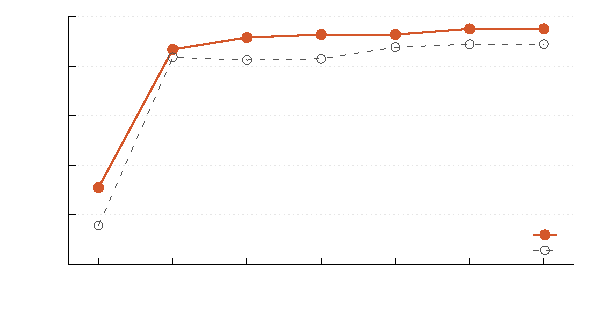
\includegraphics[width={288.00bp},height={151.00bp}]{figures/budget}}%
    \gplfronttext
  \end{picture}%
\endgroup

  \caption{Attacker with full access to the model: tasks where its target is reachable, by attack text. ``none'':
  no attack text; ``0'': the planted instruction alone; then up to that many search attempts.}
  \label{fig:budget}
\end{figure}

\begin{table}[!tb]
\centering
\small
\caption{Pre-declared comparisons on the final test, paired over 8 task types, corrected within each group.}
\label{tab:tests}
\begin{tabularx}{\columnwidth}{@{}Xl@{}}
\toprule
\textbf{Comparison} & \textbf{Result} \\
\midrule
Helper vs.\ handing over everything (unneeded authority) & $-0.80$, $p=0.008$ \\
Helper's backups vs.\ anything held (attack reach, clean / attacked) & $-65$ / $-35$ pts, $p=0.016$ \\
Helper vs.\ CAPMAS: published / retrained & $-0.55$ / $-0.37$, $p=0.039$ \\
Helper vs.\ random choice of 50\% / 75\% & $-0.36$ / $-0.60$, $p=0.039$ \\
Helper vs.\ random choice of 25\% & $-0.09$, n.s.\ (completes 12\%) \\
Benefit under each of four attacks & no significant loss \\
Fine-tuned vs.\ released, held-out families & 6 of 6 less, n.s. \\
\bottomrule
\end{tabularx}
\end{table}

\subsection{Outside benchmarks}
The ranking holds outside our tasks. On FORTIS, Qwen3-4B picks the exact least-privilege set in 40\% and 15\% of
cases on its two tasks, against 36\% and 0\% for CAPMAS and 2\% and 0\% for handing over everything. On mostargate, scored by its authors' code,
Qwen3-4B scores 0.56 against 0.26 for granting everything; larger models do better there (gpt-oss-120b 0.91).

\section{Recommendation}
\begin{itemize}
  \item \textbf{Default:} Qwen3-4B used as released, one GPU, about 0.3\,s per decision.
  \item \textbf{Alternative:} gpt-oss-120b when a few more completed tasks justify two GPUs and about 2.6\,s per
  decision.
  \item \textbf{Always} restrict later requests to the helper's backup list and keep the ceiling: the helper alone
  does not stop injected instructions.
\end{itemize}

\section{Limitations}
\begin{itemize}
  \item No helper reached our goal of 98\% of tasks completed. The main cause is that a folder missing from the first
  grant cannot be requested later.
  \item With 8 task types, large effects are clear, but similar helpers (such as Qwen3-4B and Qwen3-8B) cannot be
  separated.
  \item The fine-tuned helpers' results assume BoundClaw requests the answer fields in the same order as our client;
  this is being confirmed with the BoundClaw team.
  \item Timings are on NVIDIA L40S GPUs and will differ on other hardware.
\end{itemize}

\end{document}
